\documentclass{scrartcl}


\usepackage{amsmath,amssymb}
\usepackage{tikz}
\tikzset{node distance=2cm, auto}

\begin{document}
\small
\textbf{Topology Sheet 8, Daniel Valenzuela}

\textbf{(1)}\\
(i) A trivial line bundle gives a global trivialization. But this  gives a non-zero section and vice versa.\\
(ii) In terms of transition maps, we know that every line bundle on $S^1$ arises from the open cover of two overlapping intervals. Since $GL_1(\mathbb{R})$ has only two components, wee see that there are only two isomorphism classes of line bundles, by choosing same sign on both (there exist only two open intervals as intersection) components as transition function or different signs. And we know that there exists a non trivial line bundle, namely the Mobius band.\\
(iii) First the case of $z\mapsto z^{2n}$. Then we can look at the points in $M$ the mobiusbundle with norm 1 for a given metric. This is homeomorphic to $S^1$. The projection map $\eta$ restricts to this subspace and forms a covering space. So (the covering being two-sheeted) we can lift the loop $z\mapsto z^{2n}$ to a map $f$. By the universal property of the pullback, this defines us a section $s$:\\
\[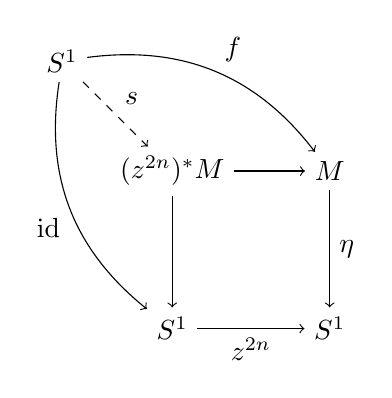
\begin{tikzpicture}
  \node (P) {$(z^{2n})^*M$};
  \node (B) [right of=P] {$M$};
  \node (A) [below of=P] {$S^1$};
  \node (C) [below of=B] {$S^1$};
  \node (P1) [node distance=1.4cm, left of=P, above of=P] {$S^1$};
  \draw[->] (P) to node {} (B);
  \draw[->] (P) to node [swap] {} (A);
  \draw[->] (A) to node [swap] {$z^{2n}$} (C);
  \draw[->] (B) to node {$\eta$} (C);
  \draw[->, bend right] (P1) to node [swap] {id} (A);
  \draw[->, bend left] (P1) to node {$f$} (B);
  \draw[->, dashed] (P1) to node {$s$} (P);
\end{tikzpicture}
\]
Vice versa a trivialization of such pullback --- or more precisely a non zero section --- would induce a map $S^1\to M \to S^1$ with even degree, therefore could not commute with a map of odd degree.

\textbf{(3)}\\
(ii) This is a special case of the easy result, that every lie group has trivial tangent bundle (and $T=S^1\times S^1$ is one). Choose neutral element $e$ and basis of the tangent space there. The topological group structure yields isomorphisms to every point's tangent space to the given basis, which satisfy a certain "local trivality" condition since it is a topological group. This is how you can extend the basis on $e$ to $n$ non-zero sections on the whole manifold (it is all the time used that group operations/inversions are smooth and depend continous).

\textbf{(4)}\\
The normal bundle of $M$ under this embedding is a 2-vector bundle. But on $S^1$ there are by the same argument as in (1) only two isomorphism classes of 2-vect bundles (pos \& neg det). Claim: the non trivial class is represented by $m \oplus l$ where $m$ for mobius and $l$ for trivial line bundle. To show the claim it suffices to show that this sum is non trivial. But this is true since otherwise the restriction (choose some metric) to the vectors of norm $1$ would yield the trivial bundle, but under the identifications coming from $m$, it is the klein bottle, which is a non trivial sphere bundle over the circle, due to non-orientability. \\
Now we conclude the triviality by saying that we know the tangent bundle of the sphere to be trivial and hence contradiction by: $\epsilon^3(S^1) = T(S^1) \oplus M = \epsilon^2 \oplus m$. (okay maybe I should have shown the claim for dimension 3 but this is similar).


\end{document}
